\chapter{Result and Discussion}
In this chapter, we discuss about the results obtained from data analysis. First, we discuss about the inclusive cross section of ${}^{17}$B. In this analysis, we extracted the inclusive 2n removal cross section and 4n removal cross section. After that, we discuss about the relative energy spectra for ${}^{16}$B +n and ${}^{15}$B + n + n at Pb and C target. Finally, the result of Coulomb dissociation and B(E1) spectrum are discussed. Dineutron correlation is also discussed in this chapter.

\section{Inclusive Cross Section}
The inclusive cross section of ${}^{17}$B of $xn$ removal reaction is obtained by following formula \cite{NKobayashi}.
\begin{align}
    \sigma_{-xn} = \frac{\sigma_R - \sigma_R'}{e^{-\sigma_R' N_t} - e^{-\sigma_R N_t}} \bigg( \frac{N'_{in}}{N_{in}} - \frac{N'_{out}}{N_{out}}\bigg),
\end{align}
where $\sigma_R$ and $\sigma_R'$ is total reaction cross section of beam and fragment particle respectively, $N_t$ is the number of target per unit area. $N_{in}$ and $N'_{in}$ are number of beam and fragment for target-in runs respectively, and $N_{out}$ and $N'_{out}$ are number of beam and fragment for target-out runs. In this research, we assume that $\sigma_R \approx \sigma_{R'}$, then the formula can be simplified as
\begin{align}
    \sigma_{-xn} &= \frac{1}{N_t} \bigg( \frac{N'_{in}}{N_{in}} - \frac{N'_{out}}{N_{out}}\bigg).
\end{align}
The calculation results of 2$n$ and 4$n$ removal cross section for each C and Pb target are shown in Table \ref{tab:Inclusive Cross Section of Boron Isotopes}. The ratio between Pb and C target is also shown in the table. The ratio of 2n removal cross section between Pb and C target was 3.9 and the ratio of 4n removal cross section was 2.4. This result is significantly smaller than the one of ${}^{19}$B, which is 7.1. This result shows that there is less Coulomb dissociation enhancement in ${}^{17}$B than ${}^{19}$B.
%We used the total reaction cross section for carbon target $\sigma_R(C)$ = 1118(22) mb\cite{Suzuki99} and for lead target $\sigma_R(Pb)$ = 4000(10) mb. 

\begin{table}[h]
\centering
\begin{tabular}{c|c|c}
    \hline
     & $\sigma_{-2n}$ (mb) & $\sigma_{-4n}$ (mb) \\
    \hline
    $^{17}$B + Pb& 618(21) & 154(11) \\ 
    $^{17}$B + C & 159(3) & 63(2) \\ 
    \hline 
    $\sigma_{Pb}/\sigma_{C}$ & 3.9 & 2.5 \\ 
    \hline
\end{tabular}
\caption{Inclusive cross section of $^{17}$B on Pb and C target}
\label{tab:Inclusive Cross Section of Boron Isotopes}
\end{table}

\section{Coulomb Dissociation Cross Section}
Coulomb dissociation cross section can be extracted by eq.(\ref{eq:CD}) from the inelastic reaction cross section for  Pb and C target. In this research, we used $\Gamma = 2.835$\cite{Ogata}. 

\begin{table}[h]
    \centering
    \begin{tabular}[h]{c|c|c}
        \hline
         &  $E{rel} < 10$ MeV&  $E{rel} < 7$ MeV \\
        \hline
        $\sigma_{inel}$(Pb) &  564(13) mb & 454(11) mb  \\
        $\sigma_{inel}$(C) &  44(1) mb & 32(1) mb  \\
        $\sigma_{\text{CD}}$ &  438(13) mb & 362(11) mb \\
        \hline
    \end{tabular}
\caption{Coulomb dissociation cross section of ${}^{17}$B}
\label{tab:CD}
\end{table}
In Figure \ref{fig:Pb+C} shows the differential cross section distribution for ${}^{15}$B $+ n + n$ on Pb and C target. The blue dot is Pb target, and red dot is C target. The C target event is scaled by $\Gamma = 2.835$ Factor. Figure \ref{fig:CD} shows the Coulomb dissociation cross section. The Coulomb dissociation cross section is 438(13) mb for $E_{rel} < 10$ MeV and 362(11) mb for $E_{rel} < 7$ MeV. It has a high and broad peak at around 2$\sim$3 MeV. 
\begin{figure}[h]
    \centering
    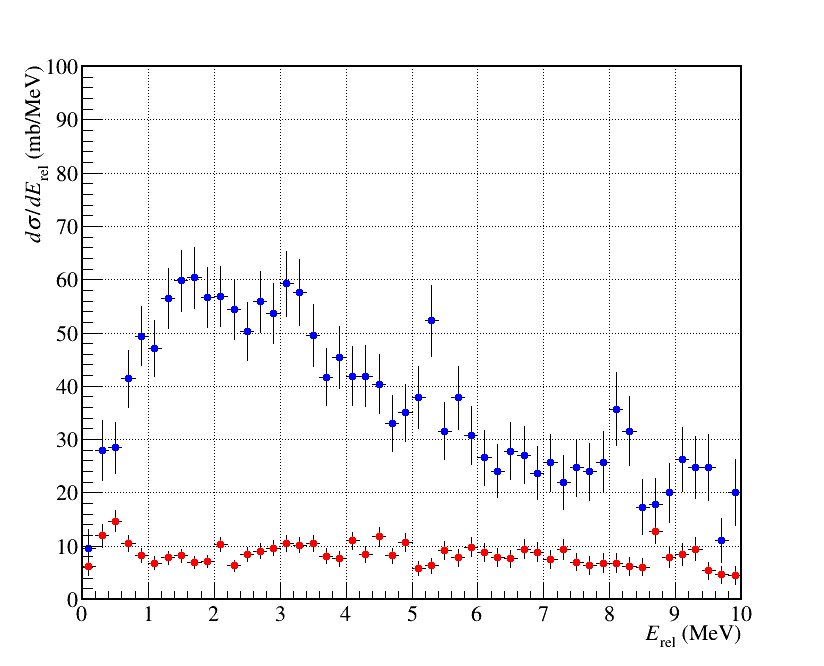
\includegraphics[width=\textwidth]{chapter5/coulomb_pb_c.png}    
    \caption[The differential cross section for ${}^{15}$B + n + n on Pb and C target]{The differential cross section for ${}^{15}$B + n + n on Pb and C target. The blue dot is Pb target, and red dot is C target. The C target event is multiplied by $\Gamma = 2.835$ factor.}
    \label{fig:Pb+C}
\end{figure}
\begin{figure}[h]
    \centering
    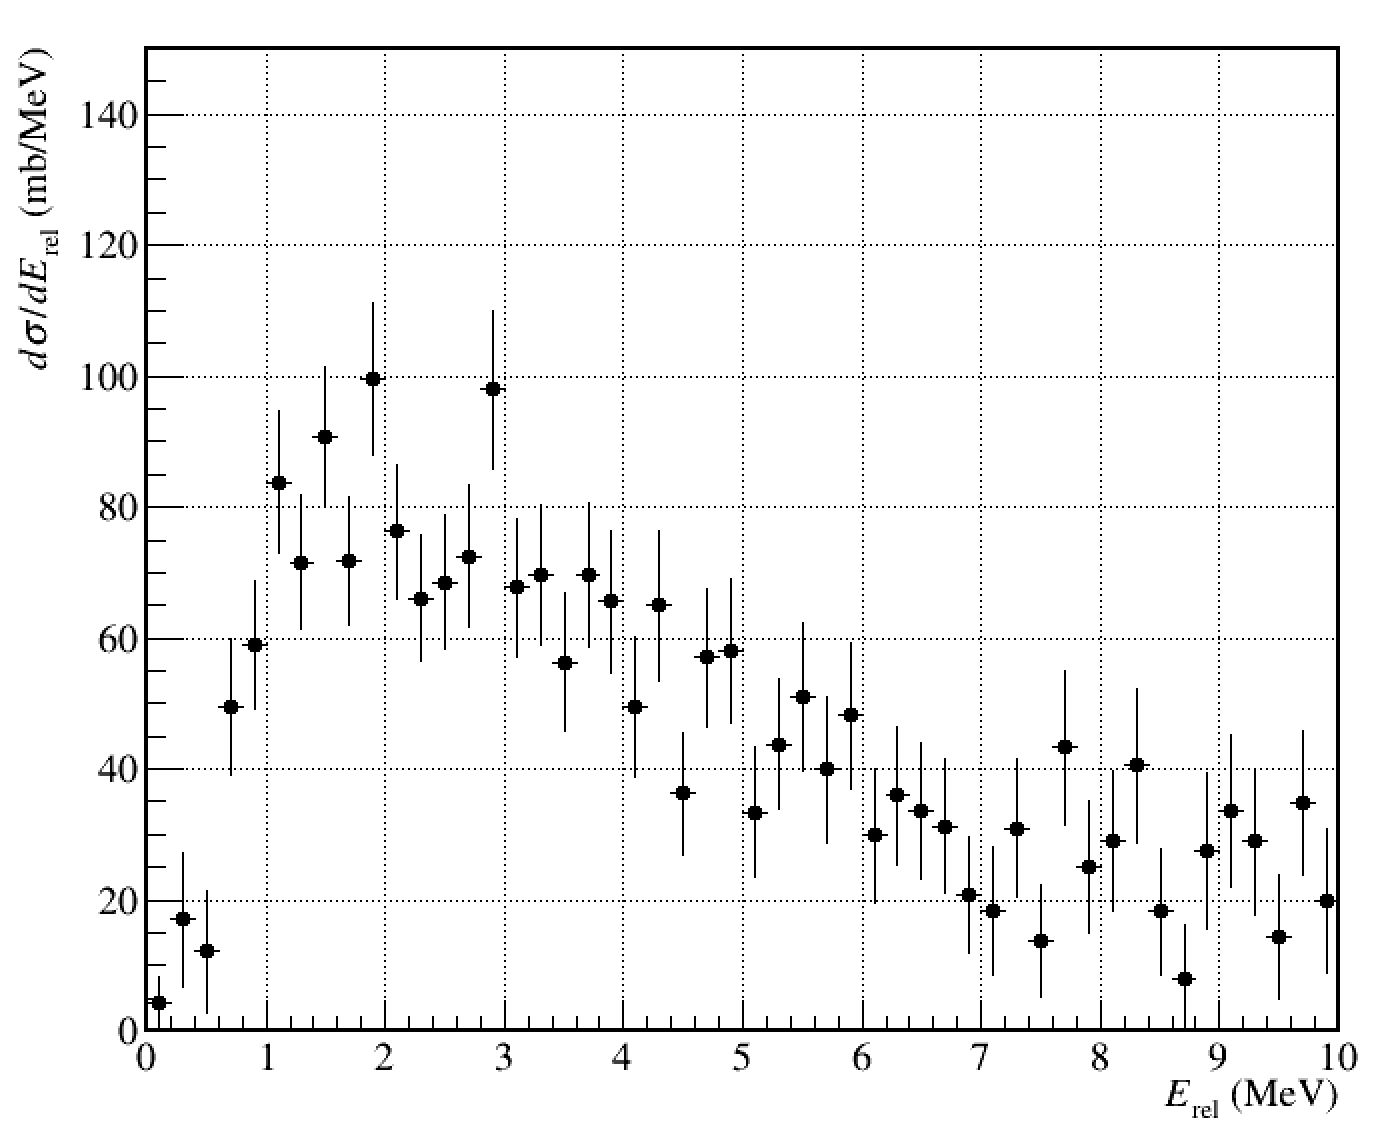
\includegraphics[width=\textwidth]{chapter5/dsigmadE.png}    
    \captionof{figure}{Coulomb dissociation cross section of ${}^{17}$B}
    \label{fig:CD}
\end{figure}    
\clearpage

\section{Reduced E1 Transition Probability}
About reduced dipole transition probability, we can extract $B(E1)$ strength as follows.
\begin{align}
    \frac{d \sigma_{coul}}{dE_x} = \frac{16 \pi^{3} }{9 \hbar c} N_{\text{E1}}(E_x) \frac{dB(\text{E1})}{dE_x}
\end{align}
The virtual photon number is calculated by using the eq.(\ref{eq:Virtual_Photon}).

\begin{figure}[h]
    \centering
    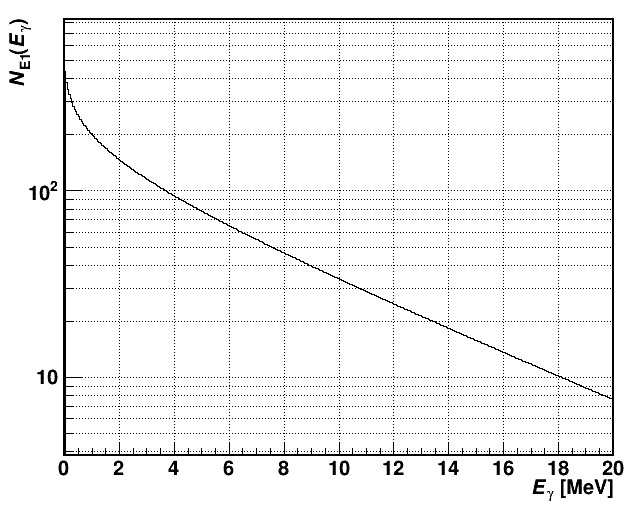
\includegraphics[width=10cm]{chapter5/virtual_photon_distribution.png}
    \captionof{figure}{Virtual Photon Number of ${}^{17}$B with 270 MeV/u at Pb Target}
\end{figure}
The reduced E1 transition probability B(E1) distribution is shown in Figure \ref{fig:B(E1)}
\begin{figure}[h]
    \centering
    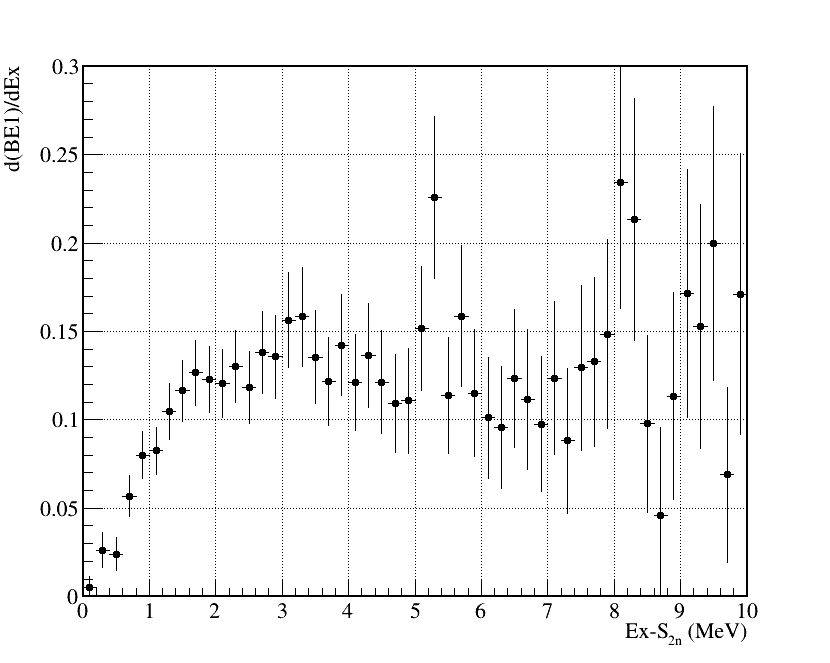
\includegraphics[width=13cm]{chapter5/dBdEx.png}    
    \captionof{figure}{B(E1) strength of ${}^{17}$B}
    \label{fig:B(E1)}
\end{figure}  

\begin{align}
    B(E1) &= \int_{0}^{+\inf} \frac{dB(E1)}{dE_x} dE_x \\
          &\simeq \int_{0}^{+10} \frac{dB(E1)}{dE_x} dE_x = 2.00 \pm 0.10  [e^{2}fm^{2}] \\
          &\simeq \int_{0}^{+7} \frac{dB(E1)}{dE_x} dE_x = 1.32 \pm 0.06  [e^{2}fm^{2}] 
\end{align}  

\section{Dineutron Correlation}
Dineutron correlation can be calculated from $B(E1)_{tot}$ as follows.
\begin{align}
    B(E1)_{tot} = \frac{3}{\pi} \bigg( \frac{Ze}{A} \bigg)^2 \langle r^{2}_{c-nn} \rangle
\end{align}
With the obtained $B(E1)$ strength up to 10 MeV and 7 MeV, we can extract $\sqrt{ \langle r^{2}_{c-nn} \rangle}$ respectively as follows.
\begin{align}
    \sqrt{ \langle r^{2}_{c-nn} \rangle} = 4.11 \pm 0.02 (stat.) \text{ fm} \qquad (0<E_{rel}<10 MeV)\\
    \sqrt{ \langle r^{2}_{c-nn} \rangle} = 3.34 \pm 0.02 (stat.) \text{ fm} \qquad (0<E_{rel}<7 MeV)
\end{align}
Furthermore, we can extract the distance of $2n$ from three body model.
\begin{align}
    \langle r^{2}_{halo} \rangle = \frac{A_c}{A} \langle r^{2}_{core} \rangle + \frac{2A_c}{A^2} \langle r^{2}_{c-nn} \rangle - \frac{1}{2A} \langle r^{2}_{nn} \rangle
\end{align}
where $A$ and $A_c$ is the mass number of halo nucleus and core. $\langle r^{2}_{h} \rangle$ and $\langle r^{2}_{c} \rangle$ are the mean-square matter radius of halo nuclei and the core, which is 3.00(6) fm and 2.75(6) fm respectively.
\begin{align}
    \sqrt{ \langle r^{2}_{nn} \rangle} &= 4.48 \pm 1.78 (stat.) \text{ fm} \qquad (0<E_{rel}<10 MeV)\\
    \sqrt{ \langle r^{2}_{nn} \rangle} &= 6.34 \pm 1.78 (stat.) \text{ fm} \qquad (0<E_{rel}<7 MeV)
\end{align}
Finally, the mean opening angle of dineutron can be extracted as follows.
\begin{align}
    \langle \theta_{nn} \rangle = 56.6 \pm 19.4 (stat.) \text{ deg.} \qquad (0<E_{rel}<10 MeV) \\
    \langle \theta_{nn} \rangle = 87.0 \pm 16.6 (stat.) \text{ deg.}\qquad (0<E_{rel}<7 MeV)
\end{align}